\chapter{Estado del Arte} % (fold)

\section{Raspberry Pi.}

Raspberry Pi es un ordenador del tamaño de una tarjeta de crédito. Consta de una placa base sobre la que se monta un procesador, un chip gráfico y memoria RAM. Fue lanzado en 2006 por la Fundación Raspberry Pi con el objeto de estimular la enseñanza de informática en las escuelas de todo el mundo.

\begin{figure}[H]
\centering
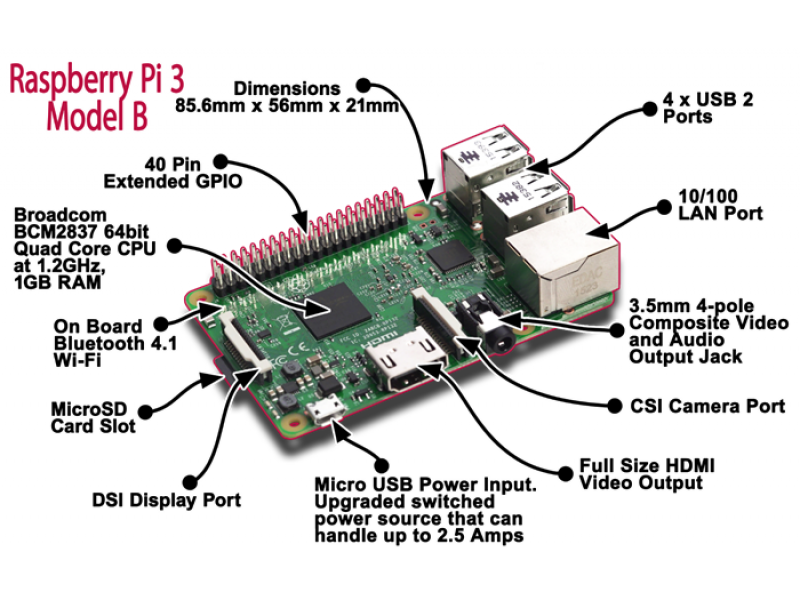
\includegraphics[width=7.5cm, height=5cm]{./images/estado-arte/raspberry.png}
\caption{Raspberry Pi 3}
\label{fig:raspberry}
\end{figure}
\\
Tiene un procesador que funciona a 700 Mhz. y puede acelerar gráficos 3D por hardware. Más o menos como el ordenador que tenías en 2003, con la salvedad de que puedes ver películas en alta definición. Se pueden instalar diversos sistemas operativos, la mayoría basados en el kernel de Linux. Algunos de los más conocidos son Android, Firefox OS, Raspbian, OpenWebOS o Unix.

\subsection{Arquitectura ARM.}
ARM es una arquitectura de 32 bits desarrollada en 1983 por la empresa Acorn Computers Ltd para usarse en computadoras personales que maneja un sistema de instrucciones realmente simple lo que le permite ejecutar tareas con un mínimo consumo de energía.
\\ 

Siendo esta razón por la que en nuestros días ha tomado bastante fuerza en el mercado de dispositivos móviles, donde el bajo consumo de energía es el objetivo primordial. La característica más interesante es el uso de los 4 bits superiores como código de condición, haciendo que cualquier instrucción pueda ser condicional.
\\

El diseño de ARM se hoy en día se ha convertido en uno de los más usados alrededor del mundo y se encuentra presente en discos duros, juguetes, móviles y tabletas. Hoy en día, cerca del 75\% de los procesadores de 32 bits poseen este chip en su núcleo. ~\cite{ARM}

\subsection{Raspian.}

Raspbian es el sistema operativo recomendado para Raspberry Pi (al estar optimizado para su hardware) y se basa en una distribución de GNU/Linux llamada Debian. La distribución es ligera para moverse ágilmente  en el hardware de la Raspberry Pi, con un entrono de escritorio LXDE y Midori como navegador web predeterminado. Además incluye herramientas de desarrollo muy interesantes. \\

 Raspbian es algo más que un sistema operativo, pues viene con unos 35 mil paquetes, precompilados, de forma tal que sea fácil instalar el que necesitemos en la Raspberry Pi.


\section{Convertidor de corriente a voltaje.}
El amplificador operacional LM324 nos permite realizar la conversión de corriente a voltaje, similar al principio del amperímetro.

\begin{figure}[H]
\centering
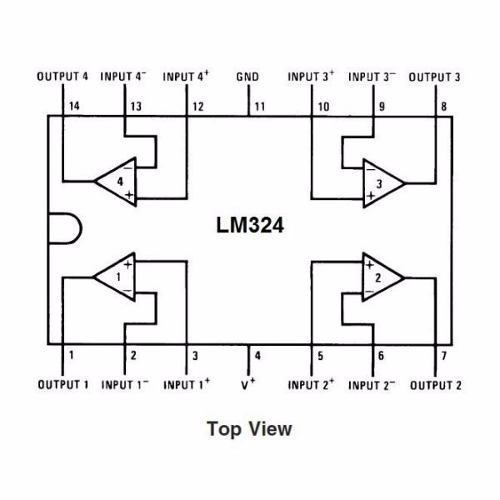
\includegraphics[width=7.5cm, height=5cm]{./images/estado-arte/LM324.jpg}
\caption{Amplificador operacional LM324}
\label{fig:lm324}
\end{figure}

\section{Servomotores.}

Un servomotor es un motor eléctrico al que podemos controlar tanto la velocidad, como la posición del eje que gira. 
\\
\begin{figure}[H]
\centering
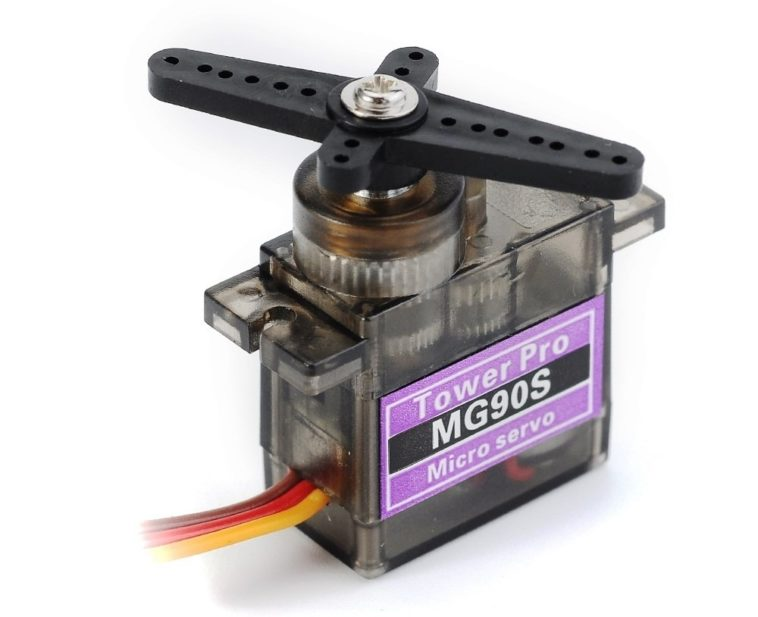
\includegraphics[width=7.5cm, height=5cm]{./images/estado-arte/servo-motor.jpg}
\caption{Servomotor}
\label{fig:servoMotor}
\end{figure}

Con los servomotores podemos crear toda clase movimientos de una forma controlada, la mayoría de los servomotores que se utilizan son de corriente continua, pero también existen en corriente alterna. \\
\begin{itemize}
    \item Características
    \begin{itemize}
        \item \textbf{El par:} También llamado torque, fuerza que es capaz de hacer en su eje.
        \item \textbf{Velocidad:} Velocidad angular de rotación.
    \end{itemize}
    
    \item Partes de un servomotor
    \begin{itemize}
        \item \textbf{Motor eléctrico:} Encargado de generar el movimiento a través de su eje.
        \item \textbf{Sistema de regulación:} Formado por engranes, que actúan sobre el motor para regular su velocidad y el par; mediante estos engranes podemos aumentar o disminuir la velocidad del par.
        \item \textbf{Sistema de control:} Circuito electrónico que controla el movimiento del motor mediante el envío de pulsos eléctricos.
        \item \textbf{Potenciómetro:} Conectado al eje central del motor que nos permite saber en todo momento el ángulo en el que se encuentra el eje del motor.
    \end{itemize}
\end{itemize}

Un pulso es sencillamente enviar corriente eléctrica al motor durante un tiempo determinado. Puedo enviar un corriente durante 0,5ms (un pulso) o durante 1,5ms (otro pulso diferente). Para el pulso de 0,5ms el eje del motor estará en una posición y para un pulso de 1,5ms el eje del motor estará en otra posición.

\begin{figure}[H]
\centering
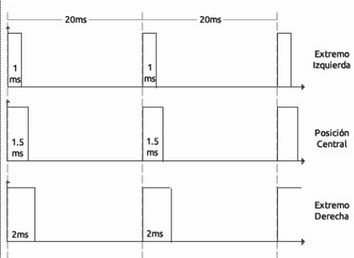
\includegraphics[width=7.5cm, height=5cm]{./images/estado-arte/pulsos-servomotores.jpg}
\caption{Pulsos en un servomotor}
\label{fig:pulsos1}
\end{figure}


\section{Lenguajes de programación.}
\subsection{Python.}
\subsection{C.}
\subsection{Android.}
Investigación de los componenentes y sistemas operativos


